%%%%%%%%%%%%%%%%%%%%%%%%%%%%%%%%%%%%%%%%%
% Programming/Coding Assignment
% LaTeX Template
%
% This template has been downloaded from:
% http://www.latextemplates.com
%
% Original author:
% Ted Pavlic (http://www.tedpavlic.com)
%
% Note:
% The \lipsum[#] commands throughout this template generate dummy text
% to fill the template out. These commands should all be removed when 
% writing assignment content.
%
% This template uses a Perl script as an example snippet of code, most other
% languages are also usable. Configure them in the "CODE INCLUSION 
% CONFIGURATION" section.
%
%%%%%%%%%%%%%%%%%%%%%%%%%%%%%%%%%%%%%%%%%

%----------------------------------------------------------------------------------------
%	PACKAGES AND OTHER DOCUMENT CONFIGURATIONS
%----------------------------------------------------------------------------------------

\documentclass{article}

\usepackage{fancyhdr} % Required for custom headers
\usepackage{lastpage} % Required to determine the last page for the footer
\usepackage{extramarks} % Required for headers and footers
\usepackage[usenames,dvipsnames]{color} % Required for custom colors
\usepackage{graphicx} % Required to insert images
\usepackage{listings} % Required for insertion of code
\usepackage{courier} % Required for the courier font
\usepackage{lipsum} % Used for inserting dummy 'Lorem ipsum' text into the template
\usepackage{setspace}
\usepackage{color}
\usepackage{comment}
\usepackage{caption}

\usepackage{hyperref}
\usepackage{natbib}
\usepackage{underscore}
\usepackage{subfigure}
\usepackage{fixltx2e}

\hypersetup{
    colorlinks=true,
    linkcolor=blue,
    filecolor=magenta,      
    urlcolor=cyan,
    breaklinks=true
}

%\usepackage[]{algorithm2e}
\usepackage{pdfpages}




%For python inclusion (http://widerin.org/blog/syntax-highlighting-for-python-scripts-in-latex-documents)
\definecolor{Code}{rgb}{0,0,0}
\definecolor{Decorators}{rgb}{0.5,0.5,0.5}
\definecolor{Numbers}{rgb}{0.5,0,0}
\definecolor{MatchingBrackets}{rgb}{0.25,0.5,0.5}
\definecolor{Keywords}{rgb}{0,0,1}
\definecolor{self}{rgb}{0,0,0}
\definecolor{Strings}{rgb}{0,0.63,0}
\definecolor{Comments}{rgb}{0,0.63,1}
\definecolor{Backquotes}{rgb}{0,0,0}
\definecolor{Classname}{rgb}{0,0,0}
\definecolor{FunctionName}{rgb}{0,0,0}
\definecolor{Operators}{rgb}{0,0,0}
\definecolor{Background}{rgb}{0.98,0.98,0.98}

% Margins
\topmargin=-0.45in
\evensidemargin=0in
\oddsidemargin=0in
\textwidth=6.5in
\textheight=9.0in
\headsep=0.25in

\linespread{1.1} % Line spacing

% Set up the header and footer
\pagestyle{fancy}
\lhead{\hmwkAuthorName} % Top left header
%\chead{\hmwkClass\ (\hmwkClassInstructor\ \hmwkClassTime): \hmwkTitle} % Top center head
\chead{\hmwkClass\ (\hmwkClassInstructor): \hmwkTitle} % Top center head
\rhead{\firstxmark} % Top right header
\lfoot{\lastxmark} % Bottom left footer
\cfoot{} % Bottom center footer
\rfoot{Page\ \thepage\ of\ \protect\pageref{LastPage}} % Bottom right footer
\renewcommand\headrulewidth{0.4pt} % Size of the header rule
\renewcommand\footrulewidth{0.4pt} % Size of the footer rule

\setlength\parindent{0pt} % Removes all indentation from paragraphs

%----------------------------------------------------------------------------------------
%	CODE INCLUSION CONFIGURATION
%----------------------------------------------------------------------------------------

\definecolor{MyDarkGreen}{rgb}{0.0,0.4,0.0} % This is the color used for comments
\lstloadlanguages{Perl} % Load Perl syntax for listings, for a list of other languages supported see: ftp://ftp.tex.ac.uk/tex-archive/macros/latex/contrib/listings/listings.pdf
\lstset{language=Perl, % Use Perl in this example
        frame=single, % Single frame around code
        basicstyle=\small\ttfamily, % Use small true type font
        keywordstyle=[1]\color{Blue}\bf, % Perl functions bold and blue
        keywordstyle=[2]\color{Purple}, % Perl function arguments purple
        keywordstyle=[3]\color{Blue}\underbar, % Custom functions underlined and blue
        identifierstyle=, % Nothing special about identifiers                                         
        commentstyle=\usefont{T1}{pcr}{m}{sl}\color{MyDarkGreen}\small, % Comments small dark green courier font
        stringstyle=\color{Purple}, % Strings are purple
        showstringspaces=false, % Don't put marks in string spaces
        tabsize=5, % 5 spaces per tab
        %
        % Put standard Perl functions not included in the default language here
        morekeywords={rand},
        %
        % Put Perl function parameters here
        morekeywords=[2]{on, off, interp},
        %
        % Put user defined functions here
        morekeywords=[3]{test},
       	%
        morecomment=[l][\color{Blue}]{...}, % Line continuation (...) like blue comment
        numbers=left, % Line numbers on left
        firstnumber=1, % Line numbers start with line 1
        numberstyle=\tiny\color{Blue}, % Line numbers are blue and small
        stepnumber=5 % Line numbers go in steps of 5
}

% Creates a new command to include a perl script, the first parameter is the filename of the script (without .pl), the second parameter is the caption
\newcommand{\perlscript}[2]{
\begin{itemize}
\item[]\lstinputlisting[caption=#2,label=#1]{#1.pl}
\end{itemize}
}


%----------------------------------------------------------------------------------------
%	DOCUMENT STRUCTURE COMMANDS
%	Skip this unless you know what you're doing
%----------------------------------------------------------------------------------------

% Header and footer for when a page split occurs within a problem environment
\newcommand{\enterProblemHeader}[1]{
\nobreak\extramarks{#1}{#1 continued on next page\ldots}\nobreak
\nobreak\extramarks{#1 (continued)}{#1 continued on next page\ldots}\nobreak
}

% Header and footer for when a page split occurs between problem environments
\newcommand{\exitProblemHeader}[1]{
\nobreak\extramarks{#1 (continued)}{#1 continued on next page\ldots}\nobreak
\nobreak\extramarks{#1}{}\nobreak
}

\setcounter{secnumdepth}{0} % Removes default section numbers
\newcounter{homeworkProblemCounter} % Creates a counter to keep track of the number of problems

\newcommand{\homeworkProblemName}{}
\newenvironment{homeworkProblem}[1][Problem \arabic{homeworkProblemCounter}]{ % Makes a new environment called homeworkProblem which takes 1 argument (custom name) but the default is "Problem #"
\stepcounter{homeworkProblemCounter} % Increase counter for number of problems
\renewcommand{\homeworkProblemName}{#1} % Assign \homeworkProblemName the name of the problem
\section{\homeworkProblemName} % Make a section in the document with the custom problem count
\enterProblemHeader{\homeworkProblemName} % Header and footer within the environment
}{
\exitProblemHeader{\homeworkProblemName} % Header and footer after the environment
}

\newcommand{\problemAnswer}[1]{ % Defines the problem answer command with the content as the only argument
\noindent\framebox[\columnwidth][c]{\begin{minipage}{0.98\columnwidth}#1\end{minipage}} % Makes the box around the problem answer and puts the content inside
}

\newcommand{\homeworkSectionName}{}
\newenvironment{homeworkSection}[1]{ % New environment for sections within homework problems, takes 1 argument - the name of the section
\renewcommand{\homeworkSectionName}{#1} % Assign \homeworkSectionName to the name of the section from the environment argument
\subsection{\homeworkSectionName} % Make a subsection with the custom name of the subsection
\enterProblemHeader{\homeworkProblemName\ [\homeworkSectionName]} % Header and footer within the environment
}{
\enterProblemHeader{\homeworkProblemName} % Header and footer after the environment
}

%----------------------------------------------------------------------------------------
%	NAME AND CLASS SECTION
%----------------------------------------------------------------------------------------
%#MOD
\newcommand{\hmwkTitle}{Assignment\ \#6 } % Assignment title
%\newcommand{\hmwkDueDate}{Monday,\ January\ 1,\ 2012} % Due date
\newcommand{\hmwkClass}{Web Science} % Course/class
%\newcommand{\hmwkClassTime}{10:30am} % Class/lecture time
\newcommand{\hmwkClassInstructor}{Alexander Nwala} % Teacher/lecturer
\newcommand{\hmwkAuthorName}{Mohd. Nauman Siddique} % Your name

%----------------------------------------------------------------------------------------
%	TITLE PAGE
%----------------------------------------------------------------------------------------

\title{
\vspace{2in}
\textmd{\textbf{\hmwkClass:\ \hmwkTitle}}\\
%\normalsize\vspace{0.1in}\small{Due\ on\ \hmwkDueDate}\\
%\vspace{0.1in}\large{\textit{\hmwkClassInstructor\ \hmwkClassTime}}
\vspace{0.1in}\large{\textit{\hmwkClassInstructor}}
\vspace{3in}
}

\author{\textbf{\hmwkAuthorName}}
%#MOD
\date{Sunday, March 31, 2019} % Insert date here if you want it to appear below your name

%----------------------------------------------------------------------------------------

\begin{document}

\maketitle



%----------------------------------------------------------------------------------------
%	TABLE OF CONTENTS
%----------------------------------------------------------------------------------------

%\setcounter{tocdepth}{1} % Uncomment this line if you don't want subsections listed in the ToC

\newpage
\tableofcontents
\newpage

\section{About the data set used in the assignment}
The goal of this project is to use the basic recommendation principles we have learned for user-collected data. You will modify the code (\url{https://github.com/arthur-e/Programming-Collective-Intelligence/blob/master/chapter2/recommendations.py}) 
given to you which performs movie recommendations from the MovieLense data sets.

The MovieLense data sets were collected by the GroupLens Research Project at the University of Minnesota during the seven-month period from September 19th, 1997 through April 22nd, 1998.  We are using the "100k dataset"; available for download from:
\url{http://grouplens.org/datasets/movielens/100k/}

There are three files which we will use:
\begin{enumerate}
\item{u.data}: 100,000 ratings by 943 users on 1,682 movies. Each user has rated at least 20 movies. Users and items are numbered
consecutively from 1. The data is randomly ordered. This is a tab separated list of 

user id | item id | rating | timestamp

The time stamps are unix seconds since 1/1/1970 UTC.

Example:

196     242     3       881250949

186     302     3       891717742

22      377     1       878887116

244     51      2       880606923

166     346     1       886397596

298     474     4       884182806

115     265     2       881171488

\item{u.item}: Information about the 1,682 movies. This is a tab
separated list of

movie id | movie title | release date | video release date | IMDb URL | unknown | Action | Adventure | Animation |Children's | Comedy | Crime | Documentary | Drama | Fantasy | Film-Noir | Horror | Musical | Mystery | Romance | Sci-Fi | Thriller | War | Western |

The last 19 fields are the genres, a 1 indicates the movie is of
that genre, a 0 indicates it is not; movies can be in several genres
at once. The movie ids are the ones used in the u.data data set.

Example:

161|Top Gun (1986)|01-Jan-1986||\url{http://us.imdb.com/M/title-exact?Top\%20Gun\%20}(1986)|0|1|0|0|0|0|0|0|0|0|0|0|0|0|1|0|0|0|0 

162|On Golden Pond (1981)|01-Jan-1981||\url{http://us.imdb.com/M/title-exact?On\%20Golden\%20Pond\%20}(1981)|0|0|0|0|0|0|0|0|1|0|0|0|0|0|0|0|0|0|0 

163|Return of the Pink Panther, The (1974)|01-Jan-1974||\url{http://us.imdb.com/M/title-exact?Return\%20of\%20the\%20Pink\%20Panther,\%20The\%20}(1974)|0|0|0|0|0|1|0|0|0|0|0|0|0|0| 0|0|0|0|0

\item{u.user}: Demographic information about the users. This is a tab
separated list of:

user id | age | gender | occupation | zip code

The user ids are the ones used in the u.data data set.

Example:

1|24|M|technician|85711 

2|53|F|other|94043 

3|23|M|writer|32067 

4|24|M|technician|43537 

5|33|F|other|15213
 \end{enumerate}
The code for reading from the u.data and u.item files and creating
recommendations is described in the book Programming Collective
Intelligence.  Feel free to modify the PCI code to answer the 
following questions.

%----------------------------------------------------------------------------------------
%	PROBLEM 1
%----------------------------------------------------------------------------------------

% To have just one problem per page, simply put a \clearpage after each problem

\begin{homeworkProblem}


 Find 3 users who are closest to you in terms of age, gender, and occupation.  For each of those 3 users:
\begin{enumerate}
\item{what are their top 3 favorite films?}
\item{bottom 3 least favorite films?}
\end{enumerate}
Based on the movie values in those 6 tables (3 users X (favorite + least)), choose a user that you feel is most like you.  Feel 
free to note any outliers (e.g., "I mostly identify with user 123, except I did not like ``Ghost'' at all").  

This user is the "substitute you".  
%\problemAnswer
%{
    \begin{verbatim}\end{verbatim}
    \textbf{SOLUTION}\\

The solution to the problem is as below:
\begin{enumerate}
 \item \textbf{Loading Movie Lens Dataset}: I read the u.data, u.user and u.item table from the Movie Lens data set and loaded them into separate json files.
\item \textbf{Find closest users }: We find the top three users that manage my category. We then find the highest rated and least rated movies for each of the three users.
\item \textbf{Most matching user}: The user 774 matches my choice of movies from all the three users. Figure \ref{SimilarUsers} shows the results for similar users anf their least favourite and most favourite movies.

\begin{lstlisting}[language=python, breaklines=true]
import json
import csv


def read_users_table():
    path_data_set = "/home/msiddique/WSDL_Work/WebScience/Assignment6/ml-100k/"
    file_open = open(path_data_set + "u.user", "r")
    list_json = []
    reader = csv.reader(file_open, delimiter="|")
    for row in reader:
        insert_row = {'user': row[0],'age': row[1],'gender': row[2],'occupation': row[3],'zip': row[4]}
        list_json.append(insert_row)
    file_json = open("Users.json", "w")
    json.dump(list_json, file_json)
    file_open.close()
    file_json.close()


def read_items_table():
    path_data_set = "/home/msiddique/WSDL_Work/WebScience/Assignment6/ml-100k/"
    # ratings = pd.read_table(path_dataset + 'u.data',sep='::',names=['user','movie','rating','time'])
    file_open = open(path_data_set + "u.item", "r", encoding = "ISO-8859-1")
    list_json = []
    reader = csv.reader(file_open, delimiter="|")
    for row in reader:
        print(row)
        insert_row = {"movie id": row[0], "movie title": row[1], "release date": row[2], "video release date": row[3],
                      "IMDb URL": row[4], "unknown": row[5], "Action": row[6], "Adventure": row[7], "Animation":row[8],
                      "Children's": row[9], "Comedy": row[10], "Crime": row[11], "Documentary": row[12],
                      "Drama": row[13], "Fantasy": row[14], "Film-Noir": row[15], "Horror": row[16], "Musical": row[17],
                      "Mystery": row[18], "Romance": row[19], "Sci-Fi": row[20], "Thriller": row[21], "War": row[22],
                      "Western": row[23]}
        list_json.append(insert_row)
    file_json = open("Items.json", "w")
    json.dump(list_json, file_json)
    file_open.close()
    file_json.close()


def read_users_data_table():
    path_data_set = "/home/msiddique/WSDL_Work/WebScience/Assignment6/ml-100k/"
    file_open = open(path_data_set + "u.data", "r")
    list_json = []
    reader = csv.reader(file_open, delimiter="\t")
    for row in reader:
        insert_row = {"user_id": row[0], "item_id": row[1], "rating": row[2], "timestamp": row[3]}
        list_json.append(insert_row)
    file_json = open("Data.json", "w")
    json.dump(list_json, file_json)
    file_open.close()
    file_json.close()


# read_users_data_table()
# read_items_table()
read_users_table()
\end{lstlisting}

\begin{lstlisting}[language=python, breaklines=true]
import json


def find_closest_user(age, occupation):
    file_json = open("Users.json", "r")
    list_json = json.load(file_json)
    list_gender = []
    for row in list_json:
        if row["gender"] == "M":
            list_gender.append(row)
    list_my_age = []
    for row in list_gender:
        if age == int(row["age"]):
            list_my_age.append(row)
    list_occupation = []
    for row in list_my_age:
        if row["occupation"] == occupation:
            list_occupation.append(row)
    if len(list_occupation) < 3:
        condition_break = False
        for row in list_my_age:
            for inner_row in list_occupation:
                if row["occupation"] != inner_row["occupation"]:
                    list_occupation.append(row)
                    condition_break = True
                    break
            if condition_break:
                break
        if len(list_occupation) < 3:
            condition_break = False
            for row in list_gender:
                for inner_row in list_occupation:
                    if row["user"] != inner_row["user"]:
                        list_occupation.append(row)
                        condition_break = True
                        break
                if condition_break:
                    break
    file_json.close()
    return list_occupation


def find_list_of_movie_ratings(age, occupation):
    list_users = find_closest_user(age, occupation)
    list_user_id = []
    for row in list_users:
        list_user_id.append(row["user"])
    file_json = open("Data.json", "r")
    list_json = json.load(file_json)
    list_favorites = []
    list_least_favourite = []
    for user in list_user_id:
        list_item_id = []
        list_ratings = []
        for row in list_json:
            if row["user_id"] == user:
                list_item_id.append(row["item_id"])
            list_ratings.append(int(row["rating"]))
        list_ratings, list_item_id = zip(*sorted(zip(list_ratings, list_item_id)))
        list_favorites.append(list_item_id[-1])
        list_least_favourite.append(list_item_id[0])
    file_json.close()
    file_json = open("Items.json", "r")
    list_json = json.load(file_json)
    list_least_favourite_movies = []
    list_favorites_movies = []
    for item_id in list_favorites:
        for row in list_json:
            if row["movie id"] == item_id:
                list_favorites_movies.append(row["movie title"])
    for item_id in list_least_favourite:
        for row in list_json:
            if row["movie id"] == item_id:
                list_least_favourite_movies.append(row["movie title"])

    for i in range(0, len(list_user_id)):
        print("For user id:" + list_user_id[i])
        print("Favorite:" + list_favorites_movies[i])
        print("Favorite movie:" + list_favorites[i])
        print("Least favorite:" + list_least_favourite[i])
        print("Least favorite movie:" + list_least_favourite_movies[i])


find_list_of_movie_ratings(30, 'student')
\end{lstlisting}


\begin{figure}[ht]
  \centering
  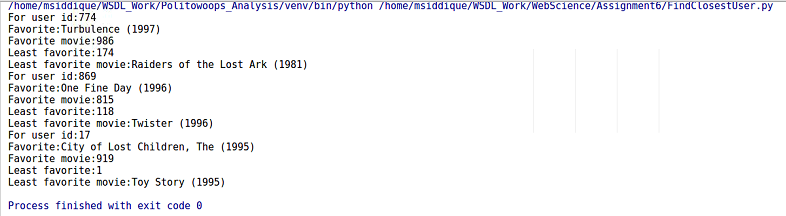
\includegraphics[width=0.9\textwidth]{S.PNG}
  \caption{Choice of most similar users to my profile}
  \label{SimilarUsers}
\end{figure}

\end{enumerate}
  
%}

\end{homeworkProblem}

%----------------------------------------------------------------------------------------
%   PROBLEM 2
%----------------------------------------------------------------------------------------

\begin{homeworkProblem}

 Which 5 users are most correlated to the substitute you? Which 5 users are least correlated (i.e., negative correlation)?
%\problemAnswer
%{
    \begin{verbatim}\end{verbatim}
    \textbf{SOLUTION}\\
For fiding correlated users, I created a json in the format shown of critics as shown in the sample recommendation code provided with the assignment. I used the json object to supply it to the function \emph{sim_pearson} from the sample recommendation code with the sustituted me and the user ids to generate the correlation values. Figure \ref{Correlation} shows the top 5 least and most correlated users.

\begin{figure}[ht]
  \centering
  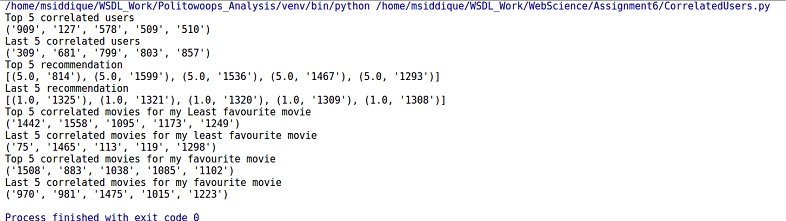
\includegraphics[width=0.9\textwidth]{Results.PNG}
  \caption{Top 5 most and least correlated users for sustitute me}
  \label{Correlation}
\end{figure}

\begin{lstlisting}[language=python, breaklines=true]
'''
Create a json file of users to mimic the critic dictionary from Recommendation.py
'''


def create_critics_json():
    file_json = open("Data.json", "r")
    list_json = json.load(file_json)
    critic ={}
    for row in list_json:
        if row["user_id"] in critic.keys():
            critic[row["user_id"]].update({row["item_id"]: int(row["rating"])})
        else:
            critic[row["user_id"]] = {row["item_id"]: int(row["rating"])}
    file_json.close()
    file_correlated_users = open("Critic.json", "w")
    json.dump(critic, file_correlated_users)
    file_correlated_users.close()


'''
Use Recommendation.py function to calculate correlation and get top 5 and last five
'''


def find_correlated_users(user_id):
    create_critics_json()
    file_json = open("Critic.json", "r")
    list_json = json.load(file_json)
    list_correlation = []
    list_user = []
    for user in list_json:
        list_user.append(user)
        list_correlation.append(sim_pearson(list_json, user_id, user))
    file_json.close()
    list_correlation, list_user = zip(*sorted(zip(list_correlation, list_user)))
    print("Top 5 correlated users")
    print(list_user[:5])
    print("Last 5 correlated users")
    print(list_user[-5:])
    get_recommended_list(user_id, list_json)
    choose_real_you(list_json)
\end{lstlisting}
%}

\end{homeworkProblem}

%----------------------------------------------------------------------------------------
%   PROBLEM 3
%----------------------------------------------------------------------------------------

\begin{homeworkProblem}

 Compute ratings for all the films that the substitute you have not seen.  Provide a list of the top 5 recommendations for films
that the substitute you should see.  Provide a list of the bottom 5 recommendations (i.e., films the substitute you is almost certain
to hate).
%\problemAnswer
%{
    \begin{verbatim}\end{verbatim}
    \textbf{SOLUTION}\\
I used the \emph{get_recommendation} function from the recommendation sample code with the json data created from the previous problem of finding correlation users with substitute me user id to get the top 5 most and meast favourite movies. Figure \ref{Recommendation} shows the resultsfor recommendation results. 

\begin{figure}[ht]
  \centering
  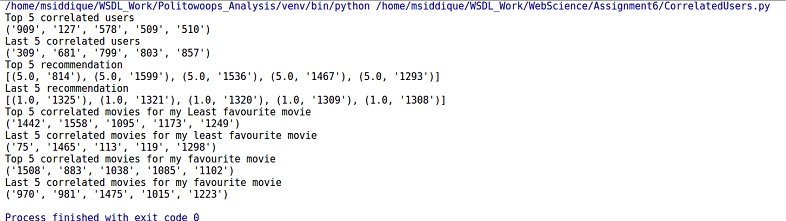
\includegraphics[width=0.9\textwidth]{Results.PNG}
  \caption{Top 5 favorite and least favorite recommendation for sustitute me user}
  \label{Recommendation}
\end{figure}

\begin{lstlisting}[language=python, breaklines=true]
'''
Function to get recommendation list for user
'''


def get_recommended_list(user_id, list_json):
    list_recommendation = getRecommendations(list_json, user_id)
    print("Top 5 recommendation")
    print(list_recommendation[:5])
    print("Last 5 recommendation")
    print(list_recommendation[-5:])
\end{lstlisting}

%}

\end{homeworkProblem}

%----------------------------------------------------------------------------------------
%   PROBLEM 4
%----------------------------------------------------------------------------------------

\begin{homeworkProblem}

Choose your (the real you, not the substitute you) favorite and
least favorite film from the data.  For each film, generate a list
of the top 5 most correlated and bottom 5 least correlated films.
Based on your knowledge of the resulting films, do you agree with
the results?  In other words, do you personally like / dislike
the resulting films?
%\problemAnswer
%{
    \begin{verbatim}\end{verbatim}
    \textbf{SOLUTION}\\
I added my favourite movie as movie id 161 (Top Gun) and least favorite movie as 162 (On Golden Pond). I added these enties into the json that I created in the correlation users case and transformed the json to be now listed by movie id rather than user id by using the function \emph{transformPrefs} from the sample recommendation code and ran the \emph{sim_pearson} function to get my list of most and least correlated top 5 movies for my favourite and least favourite movies. Figure \ref{Movie} shows the movie correlation results. 

The results for the correlation values did not make a lot of sense to me, as I had not watched many of the movies listed in the dataset. But looking at their genres and synopsis from IMDB, I realised the correlation results were very similar to my choices. 

\begin{figure}[ht]
  \centering
  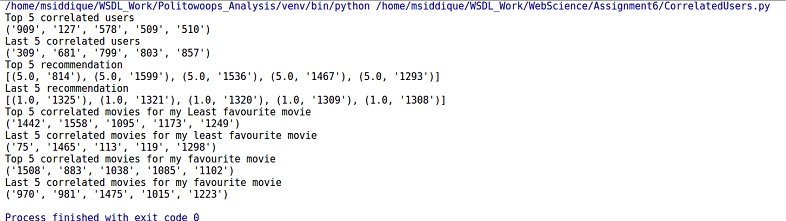
\includegraphics[width=0.9\textwidth]{Results.PNG}
  \caption{Movie Correlation for top 5 most and least correlated movies}
  \label{Movie}
\end{figure}

\begin{lstlisting}[language=python, breaklines=true]
def choose_real_you(list_json):
    list_json.update({"Me":{"161": 5, "162": 1}})
    list_transformed = transformPrefs(list_json)
    list_correlation_161 = []
    list_correlation_162 = []
    list_movies_161 = []
    list_movies_162 = []
    for movies in list_transformed:
        list_movies_161.append(movies)
        list_movies_162.append(movies)
        list_correlation_161.append(sim_pearson(list_transformed, "161", movies))
        list_correlation_162.append(sim_pearson(list_transformed, "162", movies))
    list_correlation_161, list_movies_161 = zip(*sorted(zip(list_correlation_161, list_movies_161)))
    list_correlation_162, list_movies_162 = zip(*sorted(zip(list_correlation_162, list_movies_162)))
    print("Top 5 correlated movies for my Least favourite movie")
    print(list_movies_162[:5])
    print("Last 5 correlated movies for my least favourite movie")
    print(list_movies_162[-5:])
    print("Top 5 correlated movies for my favourite movie")
    print(list_movies_161[:5])
    print("Last 5 correlated movies for my favourite movie")
    print(list_movies_161[-5:])
\end{lstlisting}

%}

\end{homeworkProblem}

\end{document}
    


   

    

    

    
   
